\chapter{Mediciones y Simulaciones}

\section{Mediciones de Parámetros (Av, Zo, Zi, Avf, Zof, Zif)}
En esta sección se presentan los resultados de las mediciones realizadas sobre el circuito implementado, tanto a lazo 
abierto como a lazo cerrado.

\begin{table}[!ht]
    \centering
    \begin{tabular}{|l|c|c|}
        \hline
        \textbf{Parámetro}  & \textbf{Valor Simulado} & \textbf{Valor Medido} \\ \hline
        $A_v$ (Lazo Abierto) & $76.5$ & $69,5$ \\ \hline
        $Z_i$ (Lazo Abierto) & $56.82 \kohm$ & [COMPLETAR] \\ \hline
        $Z_o$ (Lazo Abierto) & $1.98 \kohm$ & [COMPLETAR] \\ \hline
        $A_{vf}$ (Lazo Cerrado) & $10.75$ & $9,5$ \\ \hline
        $Z_{if}$ (Lazo Cerrado) & $182.2 \kohm$ & [COMPLETAR] \\ \hline
        $Z_{of}$ (Lazo Cerrado) & $277.41 \ohm$ & [COMPLETAR] \\ \hline
    \end{tabular}
    \caption{Comparativa de Parámetros Dinámicos}
    \label{tab:parametros}
\end{table}

\section{Medición de Desensibilidad}
Para esta prueba se provocó una variación máxima de $A_v$ del $45 \percent$, modificando un componente del 
amplificador. Las mediciones se realizaron a una frecuencia de $f_s = 1.5 \text{ kHz}$, utilizando:
\begin{itemize}
    \item $V_i = 40 \mV_{pp}$ para medir $A_v$ (Lazo Abierto).
    \item $V_{if} = 200 \mV_{pp}$ para medir $A_{vf}$ (Lazo Cerrado).
\end{itemize}

\begin{table}[!ht]
    \centering
    \begin{tabular}{|l|c|c|}
        \hline
        \textbf{Condición} & \textbf{$A_v$ (Medida)} & \textbf{$A_{vf}$ (Medida)} \\ \hline
        Original & $69,5$ & $9,5$ \\ \hline
        Con variación ($45\%$) & $31,25$ & $8,3$ \\ \hline
        \textbf{Variación Porcentual ($\Delta \percent$)} & $55\%$ & $13\%$ \\ \hline
    \end{tabular}
    \caption{Medición de Desensibilidad}
    \label{tab:desensibilidad}
\end{table}

A partir de las variaciones porcentuales obtenidas, se calcula el factor de desensibilización práctico $D$:
\begin{equation}
    D = \frac{\Delta \% A_v}{\Delta \% A_{vf}} = \frac{55\%}{13\%} = 4,23
\end{equation}

Este valor indica que, ante una degradación del $55\%$ en la ganancia de lazo abierto, la ganancia de lazo cerrado solo se vio afectada en un $13\%$, demostrando la estabilidad que aporta la realimentación negativa al sistema.

\section{Respuesta en Frecuencia}
Para la medicion de la respuesta en frecuencia del amplificador en ambos modos, se utilizaron las mismas amplitudes de
señal de entrada que para las mediciones anteriores. Solo se modificó la frecuencia de la señal. El barrido de
frecuencias que se realizo es el siguiente:

\begin{table}[!ht]
    \centering
    \begin{tabular}{|c|c|c|}
        \hline
        \textbf{Frecuencia} & \textbf{$A_v$ (LA)} & \textbf{$A_{vf}$ (LC)} \\ \hline
        $10 \si{\hertz}$        & & \\ \hline
        $50 \si{\hertz}$        & & \\ \hline
        $100 \si{\hertz}$       & & \\ \hline
        $200 \si{\hertz}$       & & \\ \hline
        $500 \si{\hertz}$       & & \\ \hline
        $800 \si{\hertz}$       & & \\ \hline
        $1 \si{\kilo\hertz}$    & & \\ \hline
        $1.5 \si{\kilo\hertz}$  & & \\ \hline
        $2 \si{\kilo\hertz}$    & & \\ \hline
        $5 \si{\kilo\hertz}$    & & \\ \hline
        $8 \si{\kilo\hertz}$    & & \\ \hline
        $10 \si{\kilo\hertz}$   & & \\ \hline
        $50 \si{\kilo\hertz}$   & & \\ \hline
        $100 \si{\kilo\hertz}$  & & \\ \hline
        $200 \si{\kilo\hertz}$  & & \\ \hline
        $400 \si{\kilo\hertz}$  & & \\ \hline
        $500 \si{\kilo\hertz}$  & & \\ \hline
        $800 \si{\kilo\hertz}$  & & \\ \hline
        $1 \si{\mega\hertz}$    & & \\ \hline
        $1.5 \si{\mega\hertz}$  & & \\ \hline
        $2 \si{\mega\hertz}$    & & \\ \hline
    \end{tabular}
    \label{tab:rta_frec}
    \caption{Ganancias obtenidas de la respuesta en frecuencia.}
\end{table}

A modo de comparacion, en la figura \ref{fig:practico_LA_LC} se muestran las graficas de ganancia en funcion de la
frecuencia de ambos amplificadores.

\begin{figure}[!ht]
    \centering
\input{figures/fig_plot_f-resp_LA_LC_lab.tex}
    \caption{Gráfica de respuesta en frecuencia (Lazo Abierto y Lazo Cerrado).}
    \label{fig:practico_LA_LC}
\end{figure}

Se puede apreciar que la respuesta en frecuencia del amplificador a lazo abierto, es bastante acotada, pudiendo suponer
una frecuencia de corte a $1 \si{\kilo\hertz}$ y a $1 \si{\mega\hertz}$.

\section{Verificación mediante Simulación}
Haciendo uso del software de simulación, se procedió a verificar los valores de ganancia y respuesta en frecuencia 
obtenidos en el punto anterior, a partir del circuito visto en la Figura \ref{fig:circuito_ltspice}.

\begin{figure}[!ht]
    \centering
    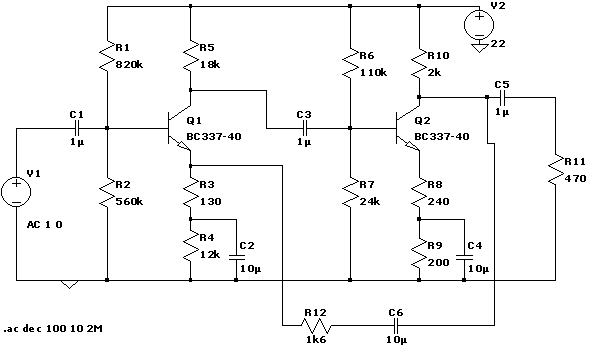
\includegraphics[width=0.8\textwidth]{images/circuito_ltspice.png}
    \caption{Circuito visto desde LTSpice.}
    \label{fig:circuito_ltspice}
\end{figure}

El comando \textbf{.ac dec 100 10 2M} hará un barrido en frecuencia de la fuente V1, de $10 \si{\hertz}$ a 
$2 \si{\mega\hertz}$

\begin{figure}[!ht]
    \centering
    \begin{tikzpicture}
    \begin{semilogxaxis}[
        width=0.9\linewidth,
        height=8cm,
        clip mode=individual,
        ylabel style={sloped like x axis, at={(0.2,1.08)} },
        xlabel={Frecuencia (Hz)},
        ylabel={Magnitud (dB)},
        grid=both,
        xmin=10, xmax=2000000,
        ymin=-4, ymax=40,
        ytick distance=4,
        extra x ticks={176.17, 772080},
        extra x tick labels={176, 772k},
        extra x tick style={grid=none, tick label style={yshift=-15pt, font=\footnotesize}}
    ]
        % Gráfica principal
        \addplot [red, thick] table [
            x index=0,
            y index=1
        ] {sources/plots/resp_freq_LA.txt};

        % Línea horizontal a -3dB (ahora arranca desde X=10)
        \addplot [black, dashed, forget plot] coordinates {(10, 34.76) (2000000, 34.76)}
            node[pos=0.965, above, font=\footnotesize] {$-3$ dB};

        % Líneas verticales
        \addplot [black, dashed, forget plot] coordinates {(176.17, 34.76) (176.17, -4)};
        \addplot [black, dashed, forget plot] coordinates {(772080, 34.76) (772080, -4)};

    \end{semilogxaxis}
\end{tikzpicture}


    \caption{Respuesta en frecuencia lazo abierto}
    \label{fig:sim_LA}
\end{figure}

Ahora hacemos el mismo analisis para el circuito a lazo cerrado, donde aumentamos el limite del barrido en la 
simulacion a $20 \si{\mega\hertz}$ para obtener un mejor resultado. Viendose en la Figura \ref{fig:sim_LC}, nuestro 
ancho de banda aumento considerablemente. Esto se logro al costo de la ganancia, la cual disminuyo al rededor de 7 veces
a la de lazo abierto. Esto se debe a que la relacion de area bajo la curva de ancho de banda, debe permanecer constante,
por lo que siempre que se aumenta el ancho de banda de alguna forma, la ganancia va a disminuir en igual proporcion al
aumento.

\begin{figure}[!ht]
    \centering
    \begin{tikzpicture}
    \begin{semilogxaxis}[
        width=0.9\linewidth,
        height=8cm,
        clip mode=individual,
        ylabel style={sloped like x axis, at={(0.2,1.08)} },
        xlabel={Frecuencia (Hz)},
        ylabel={Magnitud (dB)},
        grid=both,
        xmin=10, xmax=20000000,
        ymin=-26, ymax=25,
        ytick distance=4,
        % --- Nuevas frecuencias de corte para lazo cerrado ---
        extra x ticks={350, 6160000},
        extra x tick labels={350, 6.16M},
        extra x tick style={grid=none, tick label style={yshift=-15pt, font=\footnotesize}}
    ]
        % Gráfica principal
        \addplot [red, thick] table [
            x index=0,
            y index=1
        ] {sources/plots/resp_freq_LC.txt};

        % Línea horizontal a -3dB del nuevo máximo (20.91 - 3 = 17.91 dB)
        \addplot [black, dashed, forget plot] coordinates {(10, 17.91) (20000000, 17.91)}
            node[pos=0.964, above, font=\footnotesize] {$-3$ dB};

        % Líneas verticales bajando hasta el nuevo límite inferior (-26 dB)
        \addplot [black, dashed, forget plot] coordinates {(350, 17.91) (350, -26)};
        \addplot [black, dashed, forget plot] coordinates {(6160000, 17.91) (6160000, -26)};

    \end{semilogxaxis}
\end{tikzpicture}

    \caption{Respuesta en frecuencia lazo cerrado}
    \label{fig:sim_LC}
\end{figure}

